\documentclass{article}

% if you need to pass options to natbib, use, e.g.:
% \PassOptionsToPackage{numbers, compress}{natbib}
% before loading nips_2017
%
% to avoid loading the natbib package, add option nonatbib:
% \usepackage[nonatbib]{nips_2017}

\usepackage[final]{nips_2017}

% to compile a camera-ready version, add the [final] option, e.g.:
% \usepackage[final]{nips_2017}

\usepackage[utf8]{inputenc} % allow utf-8 input
\usepackage[T1]{fontenc}    % use 8-bit T1 fonts
\usepackage{hyperref}       % hyperlinks
\usepackage{url}            % simple URL typesetting
\usepackage{booktabs}       % professional-quality tables
\usepackage{amsfonts}       % blackboard math symbols
\usepackage{nicefrac}       % compact symbols for 1/2, etc.
\usepackage{microtype}      % microtypography
\usepackage{graphicx}
\usepackage{amsmath}

\title{Applying Compressive Sensing to the Cocktail Party Problem}

% The \author macro works with any number of authors. There are two
% commands used to separate the names and addresses of multiple
% authors: \And and \AND.
%
% Using \And between authors leaves it to LaTeX to determine where to
% break the lines. Using \AND forces a line break at that point. So,
% if LaTeX puts 3 of 4 authors names on the first line, and the last
% on the second line, try using \AND instead of \And before the third
% author name.

\author{
  Eli Saracino \\
  Department of Computer Science\\
  Boston University\\
  Boston, MA 02135 \\
  \texttt{esaracin@bu.edu} \\
  %% examples of more authors
  \And
  Andy Huynh \\
  Department of Computer Science \\
  Boston University \\
  Boston, MA 02135 \\
  \texttt{ndhuynh@bu.edu} \\
  %% \AND
  %% Coauthor \\
  %% Affiliation \\
  %% Address \\
  %% \texttt{email} \\
  %% \And
  %% Coauthor \\
  %% Affiliation \\
  %% Address \\
  %% \texttt{email} \\
  %% \And
  %% Coauthor \\
  %% Affiliation \\
  %% Address \\
  %% \texttt{email} \\
}



\begin{document}

\maketitle

\begin{abstract}
  A Compressed Sensing framework to approach blind source separation is investigated. We compare previous attempts, such as Nonnegative Matrix Factorization and Independent Component Analysis, and convey the potential advantages of Compressive Sensing: namely, it providing a more efficient reconstruction that relies far less on the necessity of learning.
\end{abstract}

\section{Introduction}
The applications of the Cocktail Party Problem are far-reaching: from surveying and separating radio signals, to imagining and examining neural signals in a medical setting, source separation plays an important role in an ever-expanding number of fields. An efficient approach to solving the Problem, then, has implications that extend far beyond the realm of Computer Science. 

Past techniques applied to solve this problem have, at a high level, relied largely on the learning of a specific dictionary, and the utilization of this dictionary to reconstruct distinct signals from potentially mixed sources. One such approach is Nonnegative Matrix Factorization, hereby NMF. As suggested, this method implies that prior information about speech sources is known in order to work properly, and, perhaps even more to its detriment, does not provide a well-defined solution in the case of over-complete dictionaries, which are so often utilized in the Compressive Sensing framework to minimize the number of measurements needed to reconstruct a given signal. \textbf{[1]} The NMF problem statement effectively tries to optimize the following cost function: 

\begin{figure}[h!]
	\centering
	
\includegraphics[width=250pt]{NMF.png}
	\label{Nonnegative Matrix Factorization}
\end{figure}

where \textbf{$\bar{D}$} is a column-wise normalized dictionary matrix and \textbf{H} is the sparse solution upon which an $L_{1}$ norm penalty is induced. In keeping with the theme of NMF, both $\bar{D}$ and \textbf{H} must be nonnegative. In the above statement, $\lambda$ is a parameter that controls the degree of sparsity.

Notably, the problem statement is not totally dissimilar to that of the standard Compressive Sensing model, albeit with some minor differences. For example, the dictionary $\bar{D}$ must be learned, usually by training on a large dataset of a single speaker. This, of course, sacrifices efficiency and casts framework of the reconstruction as a learning problem.  

With the advent of Compressive Sensing, however, we can model this problem in a new light. To do this, we first have make an assumption of sparsity; that is, in analyzing a mixed audio signal, at any given instant in time, we must assume that noise is coming from only a single source. In this way, the {\it frequency} domain of a mixed signal will be sparse, even if it should be the case that the the signal is quite robust in the time domain. With this assumption, we can frame the problem as a case of sparse signal recovery, defined as follows:

\begin{figure}[h!]
	\centering
	
\includegraphics[width=94pt, height=15pt]{compressive.png}
	\label{Compressive Sensing Problem Statement}
\end{figure}

where \textbf{S} is our set of source signals and \textbf{X} is a mixture of these signals as determined by our mixing matrix, \textbf{A}. As we will go on to show, determining \textbf{A} becomes a key step in the Compressive Sensing approach to solving the problem.

While solving this problem subject to the minimization the $L_{0}$ norm of \textbf{s} is notably NP-hard, we can obtain an approximate solution using any one of several greedy algorithms. Specifically, we apply Orthogonal Matching Pursuit to reconstruct the separate sparse signals, and transform them back into the time domain to complete the recovery.

In the coming sections, we will describe in more detail the compressive sensing approach used and it's computational benefits over such techniques as NMF, as well as some of its own shortcomings.


\section{Method}
The following is an overview of the algorithmic steps we take in applying Compressive Sensing to the Cocktail Party problem to reconstruct distinct signals from mixed input sources.

In the following steps, we'll assume we have a mixed signal of size \textit{T}. That is, there are \textit{T} discrete time instants over which our signal is heard.

In keeping with our assumption of a frequency-sparse input signal, the first step we take is to compute the Short-time Fourier transform of our source signal in order to cast it into its time-frequency domain. Shown below is a figure that demonstrates the utility of this transformation: an input signal that was originally robust becomes relatively sparse, with distinct structure forming along specific axes.

\begin{figure}[h!]
	\centering
	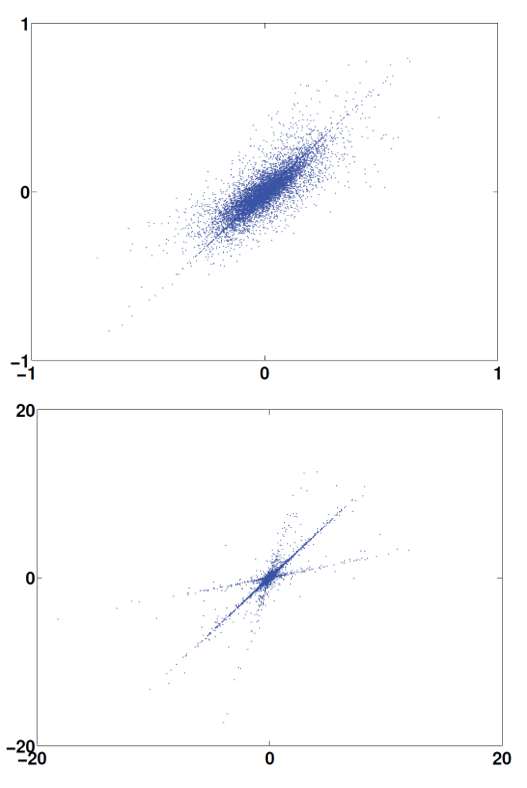
\includegraphics[width=180pt, height=220pt]{transform_domain.png}
	\caption{Above, a mixed signal in the Time domain. Below, in the Transform domain \textbf{[1]}}
	\label{Signal in each Domain}
\end{figure}

It now becomes our job to generate a mixing matrix, defined as \textbf{A} in the Introduction's problem statement, in order to create a mixture of signals, \textbf{X}, that is able to be used in the reconstruction. The first step in this process it to apply k-means clustering to the normalized STFT computed in the previous step. By setting \textit{k} to the number of original sources we hope to separate, we are able to effectively partition the frequency domain of the transformed signal along the axes defined in the above figure.

Next, we use the one-dimensional cluster centers computed from the run of k-means to construct the mixing matrix. We'll define the following notation to express this process:

Let $C = \left( \begin{smallmatrix} c_{1}&c_{2}&...&c_{\textit{k}} \end{smallmatrix} \right)$ be the cluster centers previously computed. 

Let \textit{$L_{i}$} be a \textit{T} x \textit{T} diagonal matrix, of which there are \textit{k}, and whose diagonal entries are equivalent to the corresponding \textit{$i^{th}$} entry of \textit{C} as defined above.
 
We can finally define the mixing matrix \textit{M}, then, by concatenating these matrices horizontally, as follows: $M = \left( \begin{smallmatrix} L_{1}&L_{2}&...&L_{\textit{k}}  \end{smallmatrix} \right)$

As a final preparatory step, we multiply this matrix, \textit{M}, by a \textit{T} x \textit{T} DCT matrix to further sparsify the high-frequency components of human speech \textbf{[2]}. With this step, the preparation of our problem is complete, and the reconstruction of our separated signals can begin.

In practice, the reconstruction is often performed using a windowing method,as the dimensionality of the input signal, \textit{T}, can often be quite high, and the matrices described, then, can be quite large. Choosing some \textit{l} such that you compute the mixing matrix in \textit{l} x \textit{l} sections, and use it to reconstruct partial signals in a sectionalized way is a viable strategy, and it is what we employed in our reconstructions.

At each windowing phase, we perform Orthogonal Matching Pursuit to reconstruct the portion of the signal responsible for the window being processed. The concatenation of these windows together, then, yields the full, separated, original signal.


\section{Results}
In this section, we review the results of our reconstruction and compare it to other common methods of blind source separation, analyzing the optimal window.

calculate psnr for each window size, maybe chart for best reconstruction?
results (comparison to other techniques (ICA) and NMF)

% \section{Submission of papers to NIPS 2017}
% 
% NIPS requires electronic submissions.  The electronic submission site
% is
% \begin{center}
%   \url{https://cmt.research.microsoft.com/NIPS2017/}
% \end{center}
% 
% Please read carefully the instructions below and follow them
% faithfully.
% 
% \subsection{Style}
% 
% Papers to be submitted to NIPS 2017 must be prepared according to the
% instructions presented here. Papers may only be up to eight pages
% long, including figures. This does not include acknowledgments and 
% cited references which are allowed on subsequent pages.
% Papers that exceed these limits will not be reviewed, or in any
% other way considered for presentation at the conference.
% 
% The margins in 2017 are the same as since 2007, which allow for
% $\sim$$15\%$ more words in the paper compared to earlier years.
% 
% Authors are required to use the NIPS \LaTeX{} style files obtainable
% at the NIPS website as indicated below. Please make sure you use the
% current files and not previous versions. Tweaking the style files may
% be grounds for rejection.
% 
% \subsection{Retrieval of style files}
% 
% The style files for NIPS and other conference information are
% available on the World Wide Web at
% \begin{center}
%   \url{http://www.nips.cc/}
% \end{center}
% The file \verb+nips_2017.pdf+ contains these instructions and
% illustrates the various formatting requirements your NIPS paper must
% satisfy.
% 
% The only supported style file for NIPS 2017 is \verb+nips_2017.sty+,
% rewritten for \LaTeXe{}.  \textbf{Previous style files for \LaTeX{}
%   2.09, Microsoft Word, and RTF are no longer supported!}
% 
% The new \LaTeX{} style file contains two optional arguments:
% \verb+final+, which creates a camera-ready copy, and \verb+nonatbib+,
% which will not load the \verb+natbib+ package for you in case of
% package clash.
% 
% At submission time, please omit the \verb+final+ option. This will
% anonymize your submission and add line numbers to aid review.  Please
% do \emph{not} refer to these line numbers in your paper as they will
% be removed during generation of camera-ready copies.
% 
% The file \verb+nips_2017.tex+ may be used as a ``shell'' for writing
% your paper. All you have to do is replace the author, title, abstract,
% and text of the paper with your own.
% 
% The formatting instructions contained in these style files are
% summarized in Sections \ref{gen_inst}, \ref{headings}, and
% \ref{others} below.
% 
% \section{General formatting instructions}
% \label{gen_inst}
% 
% The text must be confined within a rectangle 5.5~inches (33~picas)
% wide and 9~inches (54~picas) long. The left margin is 1.5~inch
% (9~picas).  Use 10~point type with a vertical spacing (leading) of
% 11~points.  Times New Roman is the preferred typeface throughout, and
% will be selected for you by default.  Paragraphs are separated by
% \nicefrac{1}{2}~line space (5.5 points), with no indentation.
% 
% The paper title should be 17~point, initial caps/lower case, bold,
% centered between two horizontal rules. The top rule should be 4~points
% thick and the bottom rule should be 1~point thick. Allow
% \nicefrac{1}{4}~inch space above and below the title to rules. All
% pages should start at 1~inch (6~picas) from the top of the page.
% 
% For the final version, authors' names are set in boldface, and each
% name is centered above the corresponding address. The lead author's
% name is to be listed first (left-most), and the co-authors' names (if
% different address) are set to follow. If there is only one co-author,
% list both author and co-author side by side.
% 
% Please pay special attention to the instructions in Section \ref{others}
% regarding figures, tables, acknowledgments, and references.
% 
% \section{Headings: first level}
% \label{headings}
% 
% All headings should be lower case (except for first word and proper
% nouns), flush left, and bold.
% 
% First-level headings should be in 12-point type.
% 
% \subsection{Headings: second level}
% 
% Second-level headings should be in 10-point type.
% 
% \subsubsection{Headings: third level}
% 
% Third-level headings should be in 10-point type.
% 
% \paragraph{Paragraphs}
% 
% There is also a \verb+\paragraph+ command available, which sets the
% heading in bold, flush left, and inline with the text, with the
% heading followed by 1\,em of space.
% 
% \section{Citations, figures, tables, references}
% \label{others}
% 
% These instructions apply to everyone.
% 
% \subsection{Citations within the text}
% 
% The \verb+natbib+ package will be loaded for you by default.
% Citations may be author/year or numeric, as long as you maintain
% internal consistency.  As to the format of the references themselves,
% any style is acceptable as long as it is used consistently.
% 
% The documentation for \verb+natbib+ may be found at
% \begin{center}
%   \url{http://mirrors.ctan.org/macros/latex/contrib/natbib/natnotes.pdf}
% \end{center}
% Of note is the command \verb+\citet+, which produces citations
% appropriate for use in inline text.  For example,
% \begin{verbatim}
%    \citet{hasselmo} investigated\dots
% \end{verbatim}
% produces
% \begin{quote}
%   Hasselmo, et al.\ (1995) investigated\dots
% \end{quote}
% 
% If you wish to load the \verb+natbib+ package with options, you may
% add the following before loading the \verb+nips_2017+ package:
% \begin{verbatim}
%    \PassOptionsToPackage{options}{natbib}
% \end{verbatim}
% 
% If \verb+natbib+ clashes with another package you load, you can add
% the optional argument \verb+nonatbib+ when loading the style file:
% \begin{verbatim}
%    \usepackage[nonatbib]{nips_2017}
% \end{verbatim}
% 
% As submission is double blind, refer to your own published work in the
% third person. That is, use ``In the previous work of Jones et
% al.\ [4],'' not ``In our previous work [4].'' If you cite your other
% papers that are not widely available (e.g., a journal paper under
% review), use anonymous author names in the citation, e.g., an author
% of the form ``A.\ Anonymous.''
% 
% \subsection{Footnotes}
% 
% Footnotes should be used sparingly.  If you do require a footnote,
% indicate footnotes with a number\footnote{Sample of the first
%   footnote.} in the text. Place the footnotes at the bottom of the
% page on which they appear.  Precede the footnote with a horizontal
% rule of 2~inches (12~picas).
% 
% Note that footnotes are properly typeset \emph{after} punctuation
% marks.\footnote{As in this example.}
% 
% \subsection{Figures}
% 
% All artwork must be neat, clean, and legible. Lines should be dark
% enough for purposes of reproduction. The figure number and caption
% always appear after the figure. Place one line space before the figure
% caption and one line space after the figure. The figure caption should
% be lower case (except for first word and proper nouns); figures are
% numbered consecutively.
% 
% You may use color figures.  However, it is best for the figure
% captions and the paper body to be legible if the paper is printed in
% either black/white or in color.
% \begin{figure}[h]
%   \centering
%   \fbox{\rule[-.5cm]{0cm}{4cm} \rule[-.5cm]{4cm}{0cm}}
%   \caption{Sample figure caption.}
% \end{figure}
% 
% \subsection{Tables}
% 
% All tables must be centered, neat, clean and legible.  The table
% number and title always appear before the table.  See
% Table~\ref{sample-table}.
% 
% Place one line space before the table title, one line space after the
% table title, and one line space after the table. The table title must
% be lower case (except for first word and proper nouns); tables are
% numbered consecutively.
% 
% Note that publication-quality tables \emph{do not contain vertical
%   rules.} We strongly suggest the use of the \verb+booktabs+ package,
% which allows for typesetting high-quality, professional tables:
% \begin{center}
%   \url{https://www.ctan.org/pkg/booktabs}
% \end{center}
% This package was used to typeset Table~\ref{sample-table}.
% 
% \begin{table}[t]
%   \caption{Sample table title}
%   \label{sample-table}
%   \centering
%   \begin{tabular}{lll}
%     \toprule
%     \multicolumn{2}{c}{Part}                   \\
%     \cmidrule{1-2}
%     Name     & Description     & Size ($\mu$m) \\
%     \midrule
%     Dendrite & Input terminal  & $\sim$100     \\
%     Axon     & Output terminal & $\sim$10      \\
%     Soma     & Cell body       & up to $10^6$  \\
%     \bottomrule
%   \end{tabular}
% \end{table}
% 
% \section{Final instructions}
% 
% Do not change any aspects of the formatting parameters in the style
% files.  In particular, do not modify the width or length of the
% rectangle the text should fit into, and do not change font sizes
% (except perhaps in the \textbf{References} section; see below). Please
% note that pages should be numbered.
% 
% \section{Preparing PDF files}
% 
% Please prepare submission files with paper size ``US Letter,'' and
% not, for example, ``A4.''
% 
% Fonts were the main cause of problems in the past years. Your PDF file
% must only contain Type 1 or Embedded TrueType fonts. Here are a few
% instructions to achieve this.
% 
% \begin{itemize}
% 
% \item You should directly generate PDF files using \verb+pdflatex+.
% 
% \item You can check which fonts a PDF files uses.  In Acrobat Reader,
%   select the menu Files$>$Document Properties$>$Fonts and select Show
%   All Fonts. You can also use the program \verb+pdffonts+ which comes
%   with \verb+xpdf+ and is available out-of-the-box on most Linux
%   machines.
% 
% \item The IEEE has recommendations for generating PDF files whose
%   fonts are also acceptable for NIPS. Please see
%   \url{http://www.emfield.org/icuwb2010/downloads/IEEE-PDF-SpecV32.pdf}
% 
% \item \verb+xfig+ "patterned" shapes are implemented with bitmap
%   fonts.  Use "solid" shapes instead.
% 
% \item The \verb+\bbold+ package almost always uses bitmap fonts.  You
%   should use the equivalent AMS Fonts:
% \begin{verbatim}
%    \usepackage{amsfonts}
% \end{verbatim}
% followed by, e.g., \verb+\mathbb{R}+, \verb+\mathbb{N}+, or
% \verb+\mathbb{C}+ for $\mathbb{R}$, $\mathbb{N}$ or $\mathbb{C}$.  You
% can also use the following workaround for reals, natural and complex:
% \begin{verbatim}
%    \newcommand{\RR}{I\!\!R} %real numbers
%    \newcommand{\Nat}{I\!\!N} %natural numbers
%    \newcommand{\CC}{I\!\!\!\!C} %complex numbers
% \end{verbatim}
% Note that \verb+amsfonts+ is automatically loaded by the
% \verb+amssymb+ package.
% 
% \end{itemize}
% 
% If your file contains type 3 fonts or non embedded TrueType fonts, we
% will ask you to fix it.
% 
% \subsection{Margins in \LaTeX{}}
% 
% Most of the margin problems come from figures positioned by hand using
% \verb+\special+ or other commands. We suggest using the command
% \verb+\includegraphics+ from the \verb+graphicx+ package. Always
% specify the figure width as a multiple of the line width as in the
% example below:
% \begin{verbatim}
%    \usepackage[pdftex]{graphicx} ...
%    \includegraphics[width=0.8\linewidth]{myfile.pdf}
% \end{verbatim}
% See Section 4.4 in the graphics bundle documentation
% (\url{http://mirrors.ctan.org/macros/latex/required/graphics/grfguide.pdf})
% 
% A number of width problems arise when \LaTeX{} cannot properly
% hyphenate a line. Please give LaTeX hyphenation hints using the
% \verb+\-+ command when necessary.
% 
% \subsubsection*{Acknowledgments}
% 
% Use unnumbered third level headings for the acknowledgments. All
% acknowledgments go at the end of the paper. Do not include
% acknowledgments in the anonymized submission, only in the final paper.

\section*{References}

% References follow the acknowledgments. Use unnumbered first-level
% heading for the references. Any choice of citation style is acceptable
% as long as you are consistent. It is permissible to reduce the font
% size to \verb+small+ (9 point) when listing the references. {\bf
%   Remember that you can go over 8 pages as long as the subsequent ones contain
%   \emph{only} cited references.}
\medskip

\small

[1] Schmidt, Mikkel N. and Rasmus Kongsgaard Olsson. “Single-channel speech separation using sparse non-negative matrix factorization.” {\it INTERSPEECH} (2006).

[2] BAO, G., YE, Z., XU, X. AND ZHOU, Y.
{\it A Compressed Sensing Approach to Blind Separation of Speech Mixture Based on a Two-Layer Sparsity Model} - IEEE Journals \& Magazine Bao, G., Ye, Z., Xu, X. and Zhou, Y. (2017). A Compressed Sensing Approach to Blind Separation of Speech Mixture Based on a Two-Layer Sparsity Model - IEEE Journals \& Magazine. [online] Ieeexplore.ieee.org. Available at: http://ieeexplore.ieee.org/document/6384713/
\end{document}
